\documentclass[border=10pt]{standalone}
\usepackage{amsmath}
\usepackage{amssymb}
\usepackage{tikz}
\usetikzlibrary{arrows.meta, positioning, fit, calc, shapes.geometric, backgrounds}

\begin{document}
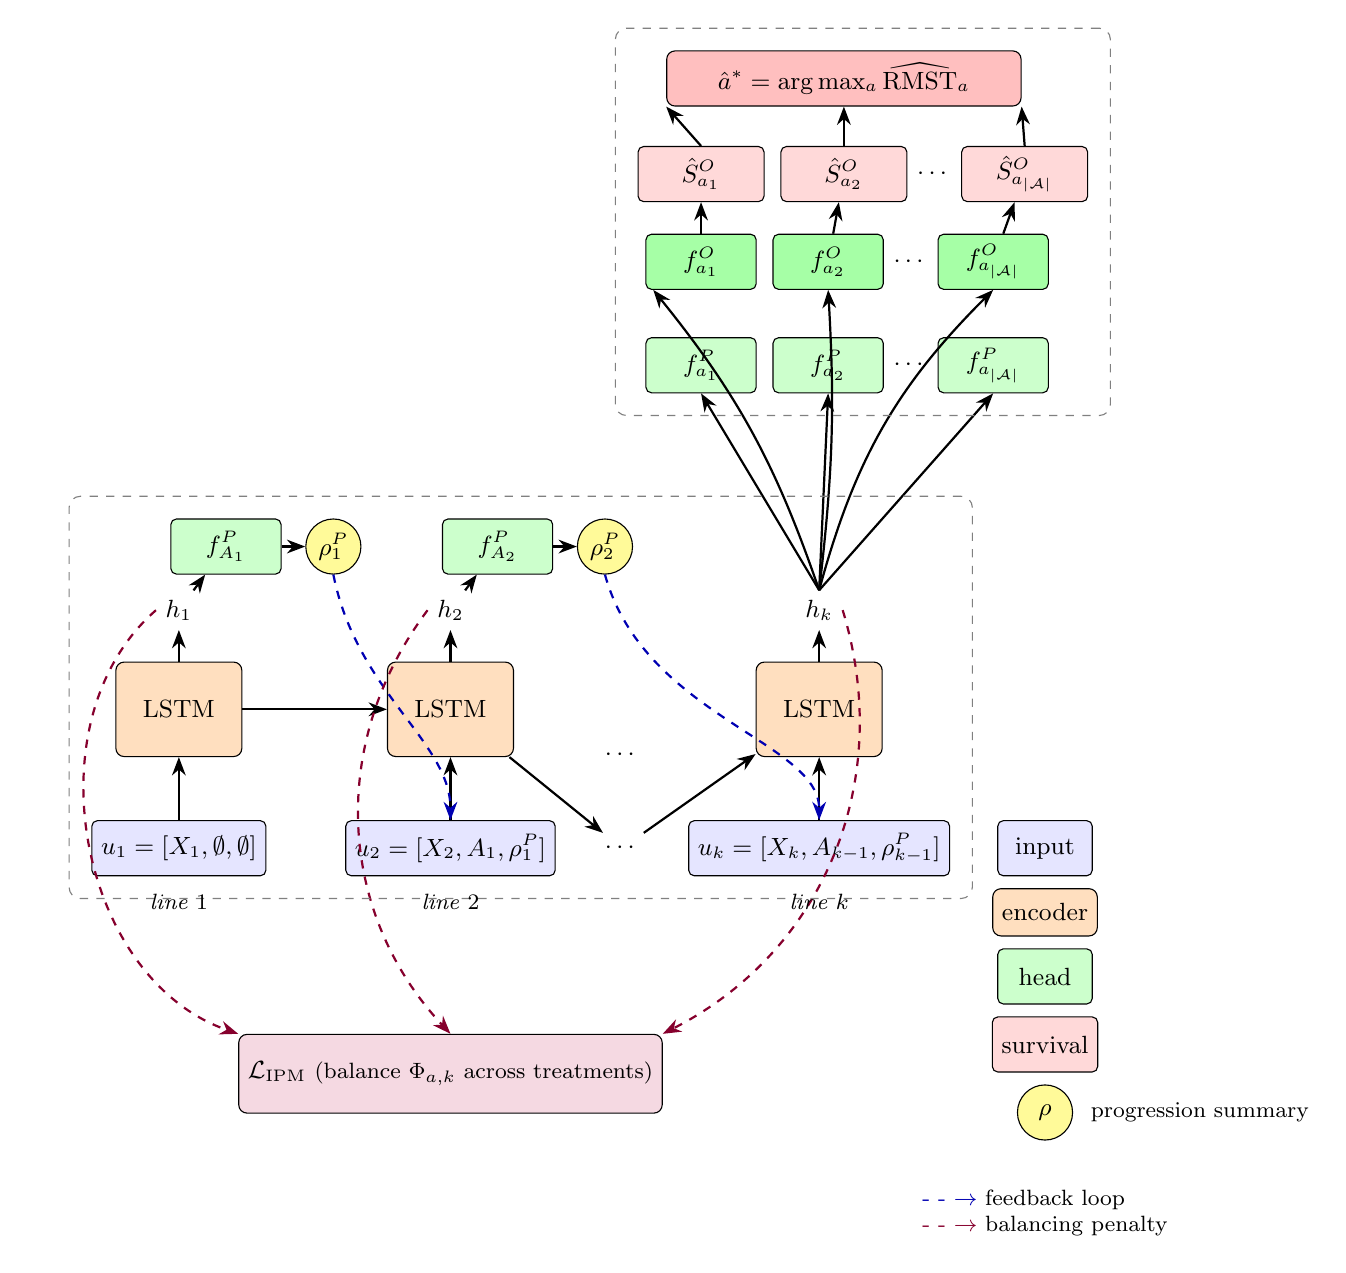
\begin{tikzpicture}[
    font=\small,
    arr/.style={-{Stealth}, thick},
    dasharr/.style={-{Stealth}, thick, dashed},
    input/.style={rectangle, draw, fill=blue!10, minimum width=1.6cm, minimum height=0.7cm, rounded corners=2pt},
    lstm/.style={rectangle, draw, fill=orange!25, minimum width=1.6cm, minimum height=1.2cm, rounded corners=3pt},
    head/.style={rectangle, draw, fill=green!20, minimum width=1.4cm, minimum height=0.7cm, rounded corners=2pt},
    output/.style={rectangle, draw, fill=red!15, minimum width=1.6cm, minimum height=0.7cm, rounded corners=2pt},
    rho/.style={circle, draw, fill=yellow!40, minimum size=0.7cm, inner sep=1pt},
    label/.style={font=\footnotesize\itshape},
]

% ============ Time step j-1 ============
\node[input] (u1) at (0, 0) {$u_{1} = [X_1, \emptyset, \emptyset]$};
\node[input, right=1.0cm of u1] (u2) {$u_{2} = [X_2, A_1, \rho^P_1]$};
\node[right=0.5cm of u2] (dots1) {$\cdots$};
\node[input, right=0.5cm of dots1] (uk) {$u_k = [X_k, A_{k-1}, \rho^P_{k-1}]$};

% LSTM cells
\node[lstm, above=0.8cm of u1] (lstm1) {LSTM};
\node[lstm, above=0.8cm of u2] (lstm2) {LSTM};
\node[above=0.8cm of dots1] (lstmdots) {$\cdots$};
\node[lstm, above=0.8cm of uk] (lstmk) {LSTM};

% Hidden states
\node[above=0.4cm of lstm1] (h1) {$h_1$};
\node[above=0.4cm of lstm2] (h2) {$h_2$};
\node[above=0.4cm of lstmk] (hk) {$h_k$};

% Progression heads (auxiliary, feeding back)
\node[head, above right=0.2cm and -0.4cm of h1] (fp1) {$f^P_{A_1}$};
\node[rho, right=0.3cm of fp1] (rho1) {$\rho^P_1$};

\node[head, above right=0.2cm and -0.4cm of h2] (fp2) {$f^P_{A_2}$};
\node[rho, right=0.3cm of fp2] (rho2) {$\rho^P_2$};

% Inputs to LSTM
\draw[arr] (u1) -- (lstm1);
\draw[arr] (u2) -- (lstm2);
\draw[arr] (uk) -- (lstmk);

% LSTM horizontal recurrence
\draw[arr] (lstm1) -- (lstm2);
\draw[arr] (lstm2) -- (dots1);
\draw[arr] (dots1) -- (lstmk);

% LSTM to hidden states
\draw[arr] (lstm1) -- (h1);
\draw[arr] (lstm2) -- (h2);
\draw[arr] (lstmk) -- (hk);

% Hidden states to progression heads
\draw[arr] (h1) -- (fp1);
\draw[arr] (h2) -- (fp2);
\draw[arr] (fp1) -- (rho1);
\draw[arr] (fp2) -- (rho2);

% Feedback loop: rho fed into next u
\draw[dasharr, blue!70!black] (rho1.south) .. controls +(0.3,-1.5) and +(0,1.0) .. (u2.north);
\draw[dasharr, blue!70!black] (rho2.south) .. controls +(0.5,-1.8) and +(0,1.0) .. (uk.north);

% ============ Decision point at line k ============
% Treatment-specific heads at line k
\node[head, above=2.5cm of hk, xshift=-1.5cm] (fpk_a1) {$f^P_{a_1}$};
\node[head, right=0.2cm of fpk_a1] (fpk_a2) {$f^P_{a_2}$};
\node[right=0.0cm of fpk_a2] (fpk_dots) {$\cdots$};
\node[head, right=0.0cm of fpk_dots] (fpk_aA) {$f^P_{a_{|\mathcal{A}|}}$};

\node[head, above=0.6cm of fpk_a1, fill=green!35] (fok_a1) {$f^O_{a_1}$};
\node[head, right=0.2cm of fok_a1, fill=green!35] (fok_a2) {$f^O_{a_2}$};
\node[right=0.0cm of fok_a2] (fok_dots) {$\cdots$};
\node[head, right=0.0cm of fok_dots, fill=green!35] (fok_aA) {$f^O_{a_{|\mathcal{A}|}}$};

% h_k to all heads at line k
\draw[arr] (hk.north) -- ($(fpk_a1.south)+(0,0)$);
\draw[arr] (hk.north) -- ($(fpk_a2.south)+(0,0)$);
\draw[arr] (hk.north) -- ($(fpk_aA.south)+(0,0)$);
\draw[arr] (hk.north) to[bend right=10] ($(fok_a1.south west)+(0.1,0)$);
\draw[arr] (hk.north) to[bend right=5]  ($(fok_a2.south)+(0,0)$);
\draw[arr] (hk.north) to[bend left=15]  ($(fok_aA.south)+(0,0)$);

% Outputs
\node[output, above=0.4cm of fok_a1] (Sk_a1) {$\hat{S}^O_{a_1}$};
\node[output, right=0.2cm of Sk_a1] (Sk_a2) {$\hat{S}^O_{a_2}$};
\node[right=0.0cm of Sk_a2] (Sk_dots) {$\cdots$};
\node[output, right=0.0cm of Sk_dots] (Sk_aA) {$\hat{S}^O_{a_{|\mathcal{A}|}}$};

\draw[arr] (fok_a1) -- (Sk_a1);
\draw[arr] (fok_a2) -- (Sk_a2);
\draw[arr] (fok_aA) -- (Sk_aA);

% RMST argmax box
\node[rectangle, draw, fill=red!25, rounded corners=3pt, above=0.5cm of Sk_a2, minimum width=4.5cm, minimum height=0.7cm] (rmst) {$\hat{a}^* = \arg\max_a \widehat{\text{RMST}}_a$};
\draw[arr] (Sk_a1.north) -- (rmst.south west);
\draw[arr] (Sk_a2.north) -- (rmst.south);
\draw[arr] (Sk_aA.north) -- (rmst.south east);

% IPM regularizer (acting on h_k across treatments in batch)
\node[rectangle, draw, fill=purple!15, rounded corners=3pt, below=2.0cm of u2, minimum width=3.5cm, minimum height=1.0cm, align=center] (ipm) {$\mathcal{L}_{\text{IPM}}$ \footnotesize (balance $\Phi_{a,k}$ across treatments)};
\draw[dasharr, purple!70!black] (h1.west) to[bend right=60] (ipm.north west);
\draw[dasharr, purple!70!black] (h2.west) to[bend right=40] (ipm.north);
\draw[dasharr, purple!70!black] (hk.east) to[bend left=40] (ipm.north east);

% Encoder bracket
\node[draw, dashed, gray, rounded corners=4pt, fit=(u1)(uk)(lstm1)(lstmk)(h1)(hk)(fp1)(fp2)(rho1)(rho2), inner sep=8pt, label={[gray, font=\small\bfseries]below:Shared encoder $\phi$}] {};

% Decision point bracket
\node[draw, dashed, gray, rounded corners=4pt, fit=(fpk_a1)(fpk_aA)(fok_a1)(fok_aA)(Sk_a1)(Sk_aA)(rmst), inner sep=8pt, label={[gray, font=\small\bfseries]right:Decision at line $k$}] {};

% Time step labels
\node[label, below=0.1cm of u1] {line $1$};
\node[label, below=0.1cm of u2] {line $2$};
\node[label, below=0.1cm of uk] {line $k$};

% Legend
\begin{scope}[shift={(11, 0)}]
    \node[input, minimum width=1.2cm] (leg_in) at (0, 0) {input};
    \node[lstm, minimum width=1.2cm, minimum height=0.6cm, below=0.15cm of leg_in] (leg_lstm) {encoder};
    \node[head, minimum width=1.2cm, below=0.15cm of leg_lstm] (leg_head) {head};
    \node[output, minimum width=1.2cm, below=0.15cm of leg_head] (leg_out) {survival};
    \node[rho, below=0.15cm of leg_out] (leg_rho) {$\rho$};
    \node[right=0.1cm of leg_rho, font=\footnotesize] {progression summary};

    \node[font=\footnotesize, align=left, below=0.5cm of leg_rho] {
        \textcolor{blue!70!black}{- - $\rightarrow$} feedback loop\\
        \textcolor{purple!70!black}{- - $\rightarrow$} balancing penalty
    };
\end{scope}

\end{tikzpicture}
\end{document}